%%
%% This is file `expeg.tex',
%% generated with the docstrip utility.
%%
%% The original source files were:
%%
%% expressg.dtx  (with options: `egt')
%% 
%%   Author: Peter Wilson (CUA) now at peter.r.wilson@boeing.com until June 2004
%%                              (or pandgwilson@earthlink.net)
%%   Copyright 1996, 2003 Peter R. Wilson
%% 
%%  v1.0 1996/05/09 (first release)
%%  v1.2 1999/11/15
%%  v1.3 2000/05/22
%%  v1.4 2000/07/10
%%  v1.5 2003/07/31
%%  v1.6 2004/02/29
%%  v1.61 2004/03/17
%% 
%%   This work may be distributed and/or modified under the
%%   conditions of the LaTeX Project Public License, either
%%   version 1.3 of this license or (at your option) any
%%   later version.
%%   The latest version of the license is in
%%      http://www.latex-project.org/lppl.txt
%%   and version 1.3 or later is part of all distributions of
%%   LaTeX version 2003/06/01 or later.
%% 
%%   This work has the LPPL maintenance status "author-maintained".
%% 
%%   This work consists of the files listed in the README file.
%%  This program is provided under the terms of the
%%  LaTeX Project Public License distributed from CTAN
%%  archives in directory macros/latex/base/lppl.txt.
%% 
%%% expeg.tex    display expressg.dtx MetaPost examples

\documentclass[11pt]{article}
\newif\ifpdf
\ifx\pdfoutput\undefined
  \pdffalse
\else
  \pdftrue
\fi

\ifpdf
  \pdfoutput=1
  \usepackage[pdftex,final]{graphicx}
  \DeclareGraphicsRule{*}{mps}{*}{}
\else
  \usepackage[final]{graphicx}
\fi

%%%% page sizes for ISO document on A4 paper
\setlength{\headheight}{11pt}
\setlength{\headsep}{10mm}
\setlength{\topskip}{11pt}
\setlength{\footskip}{11mm}
\setlength{\textwidth}{160mm}
\setlength{\textheight}{221.5mm}
\setlength{\columnsep}{10mm}
\setlength{\topmargin}{0mm}
\setlength{\oddsidemargin}{0mm}
\setlength{\evensidemargin}{0mm}
\setlength{\marginparwidth}{0pt}
\setlength{\marginparsep}{0pt}
\setlength{\marginparpush}{0pt}
\setlength{\footnotesep}{12pt}
  %%%% for US letterpaper need to change some margins
\setlength{\topmargin}{-9.4mm}
\setlength{\oddsidemargin}{1.55mm}
\setlength{\evensidemargin}{1.55mm}

\begin{document}

\begin{figure}
\centering
  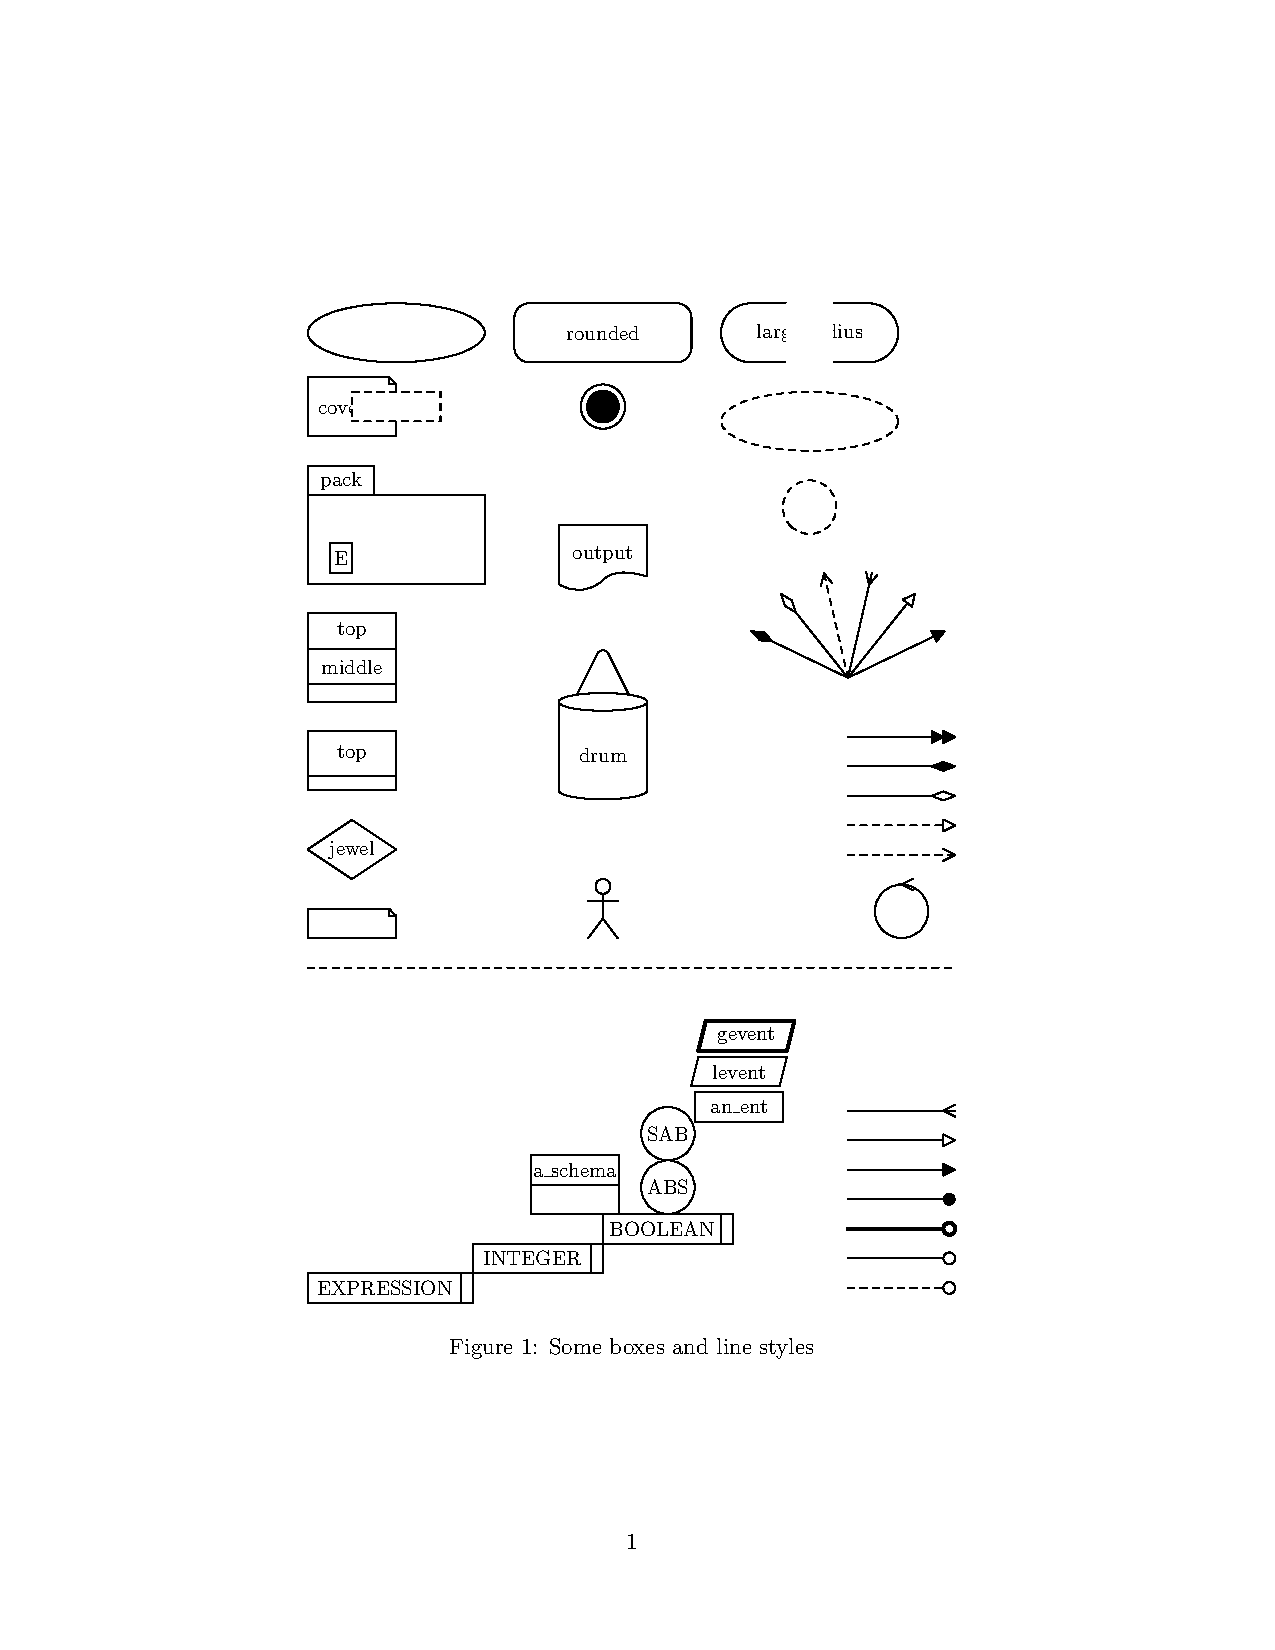
\includegraphics{expeg.1}
\caption{Some boxes and line styles}
\end{figure}

\begin{figure}
\centering
  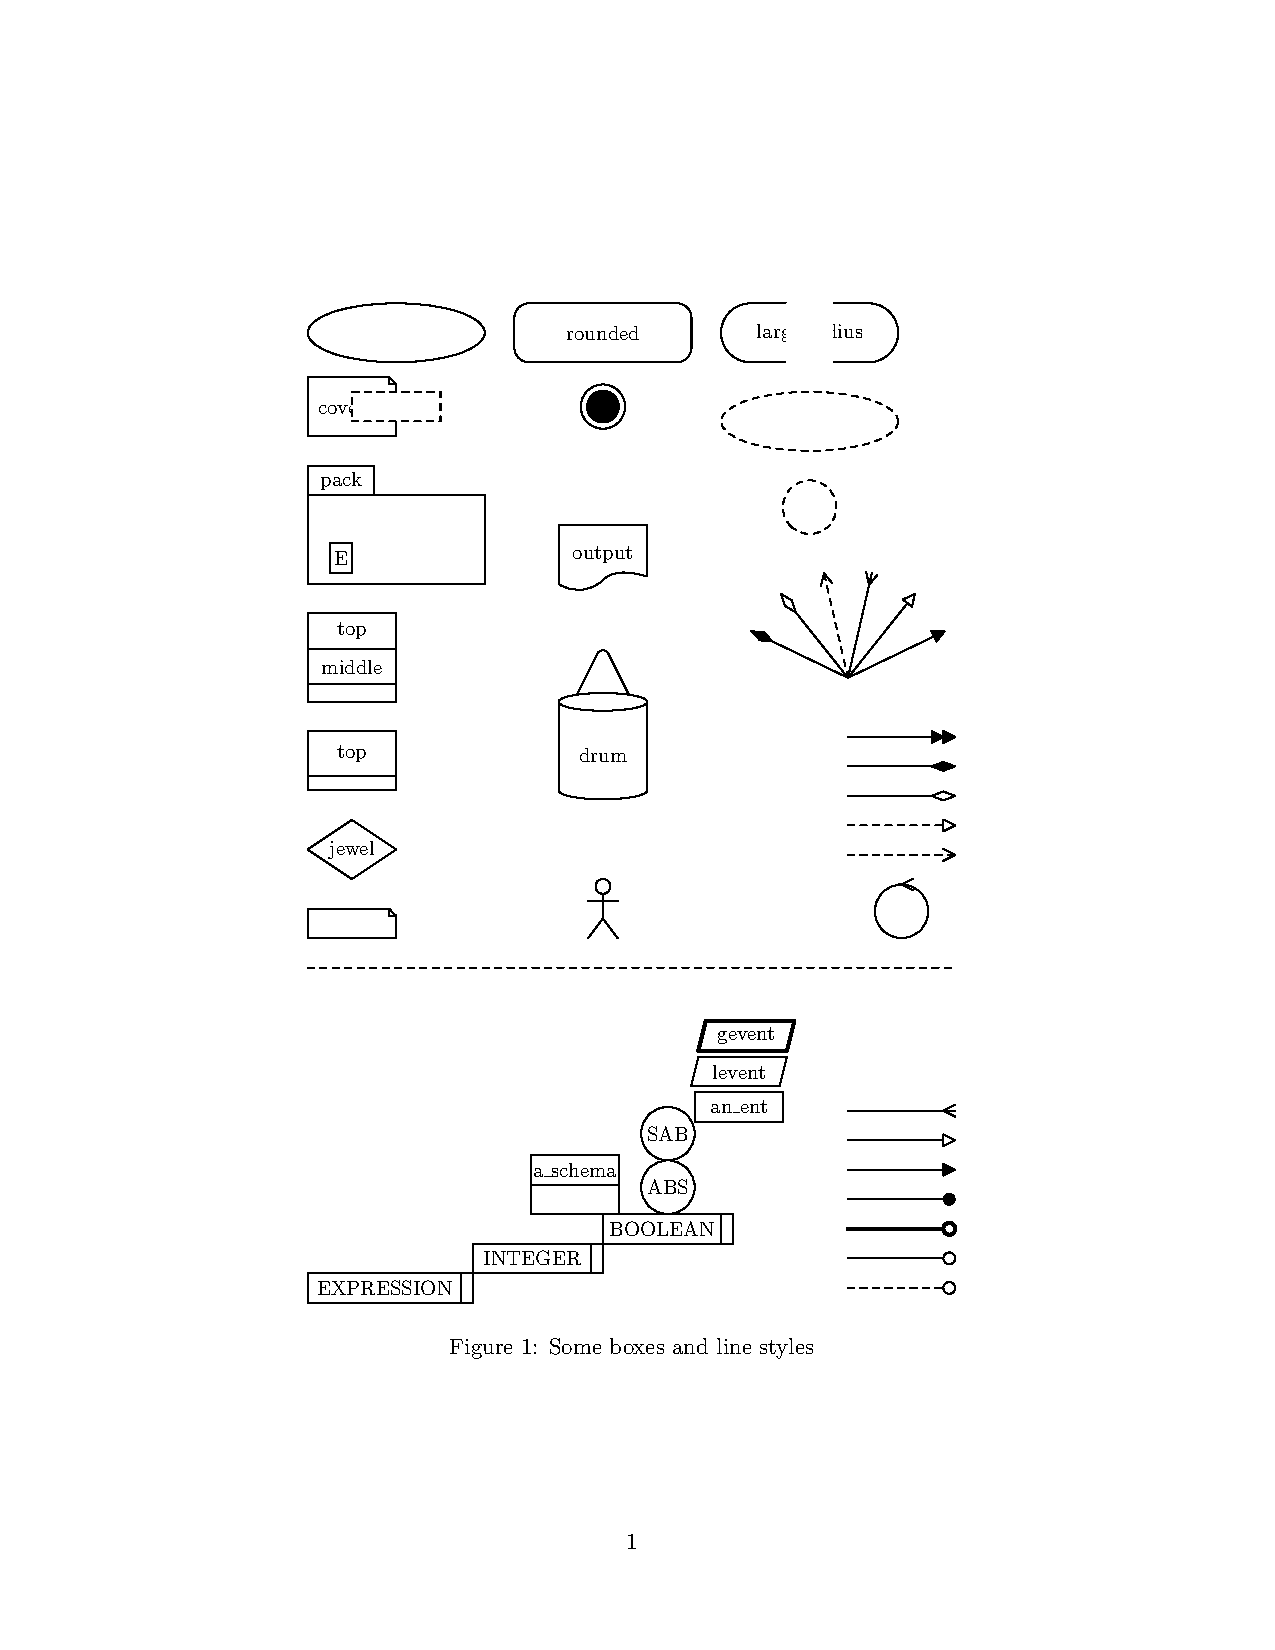
\includegraphics{expeg.2}
\caption{Example schema level diagram}
\end{figure}

\begin{figure}
\centering
  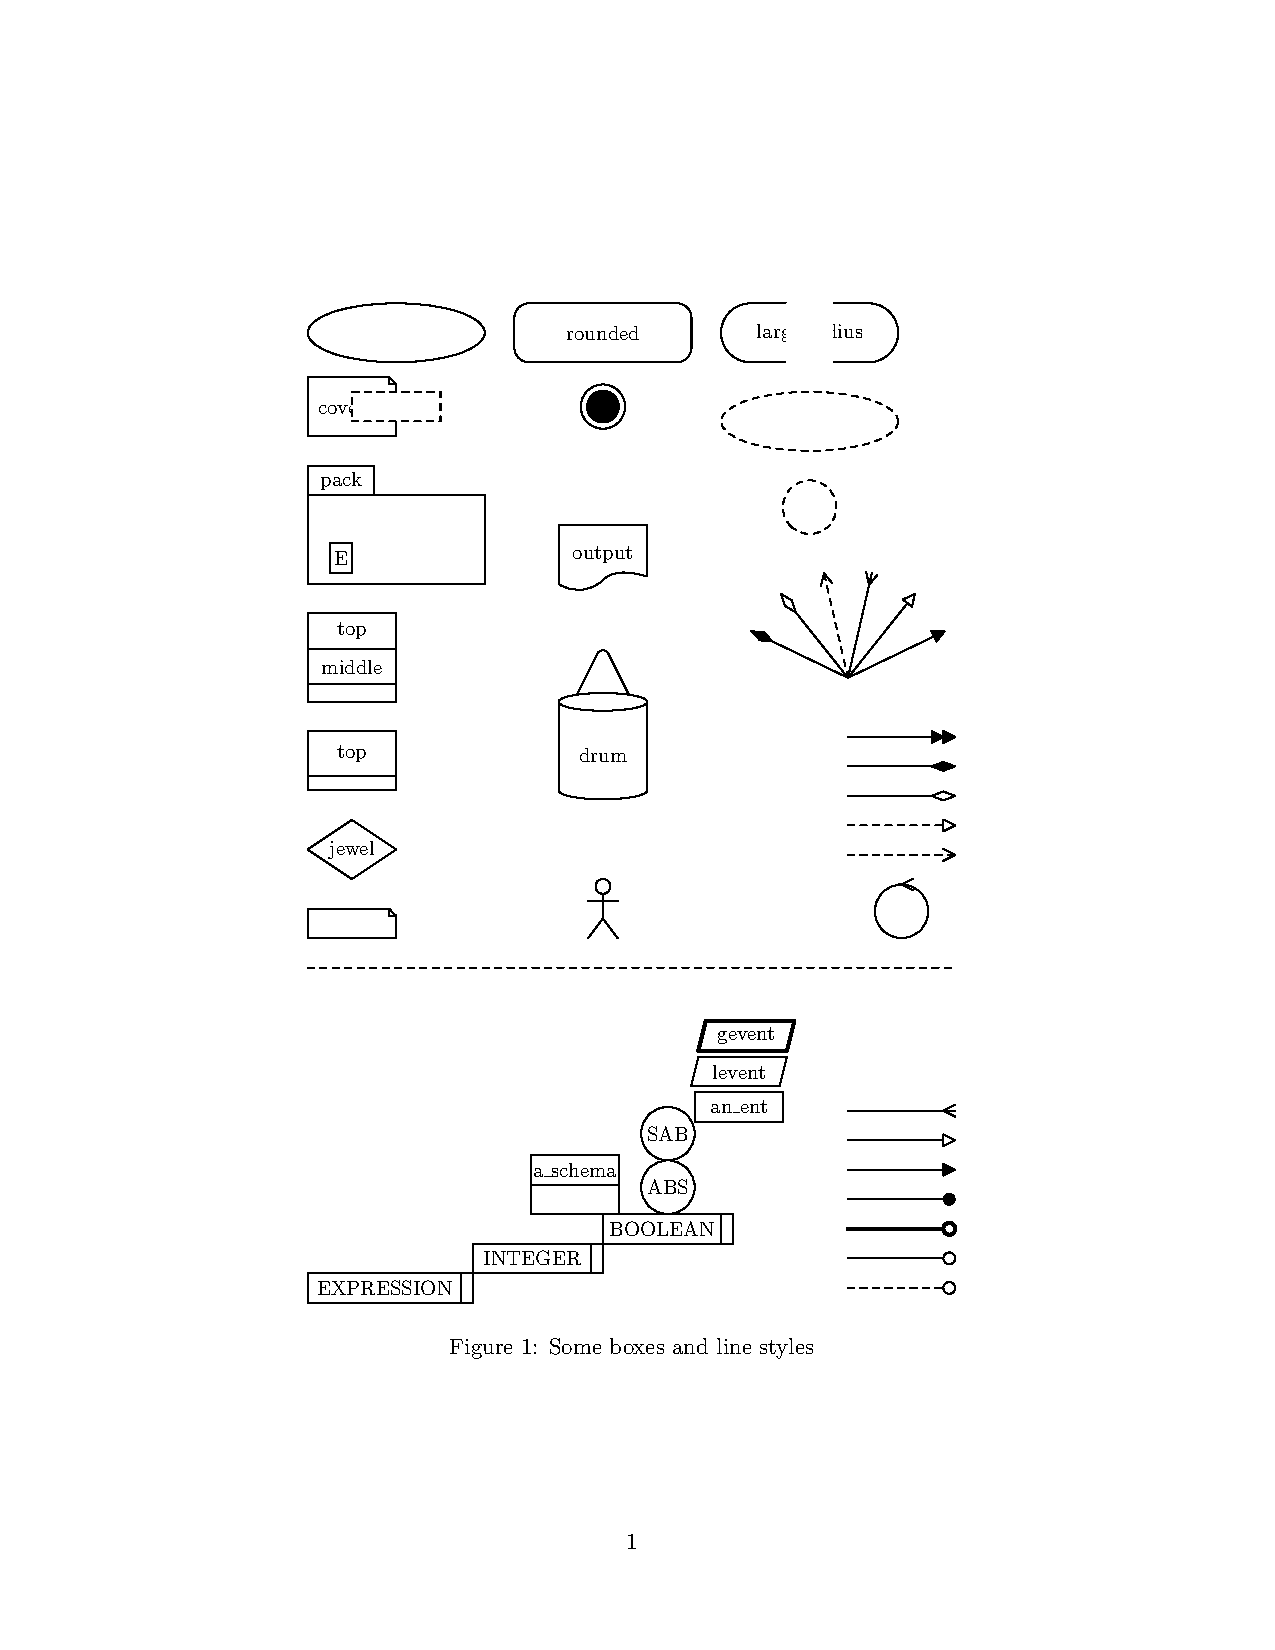
\includegraphics{expeg.3}
\caption{Example diagram of a tree structure}
\end{figure}

\begin{figure}
\centering
  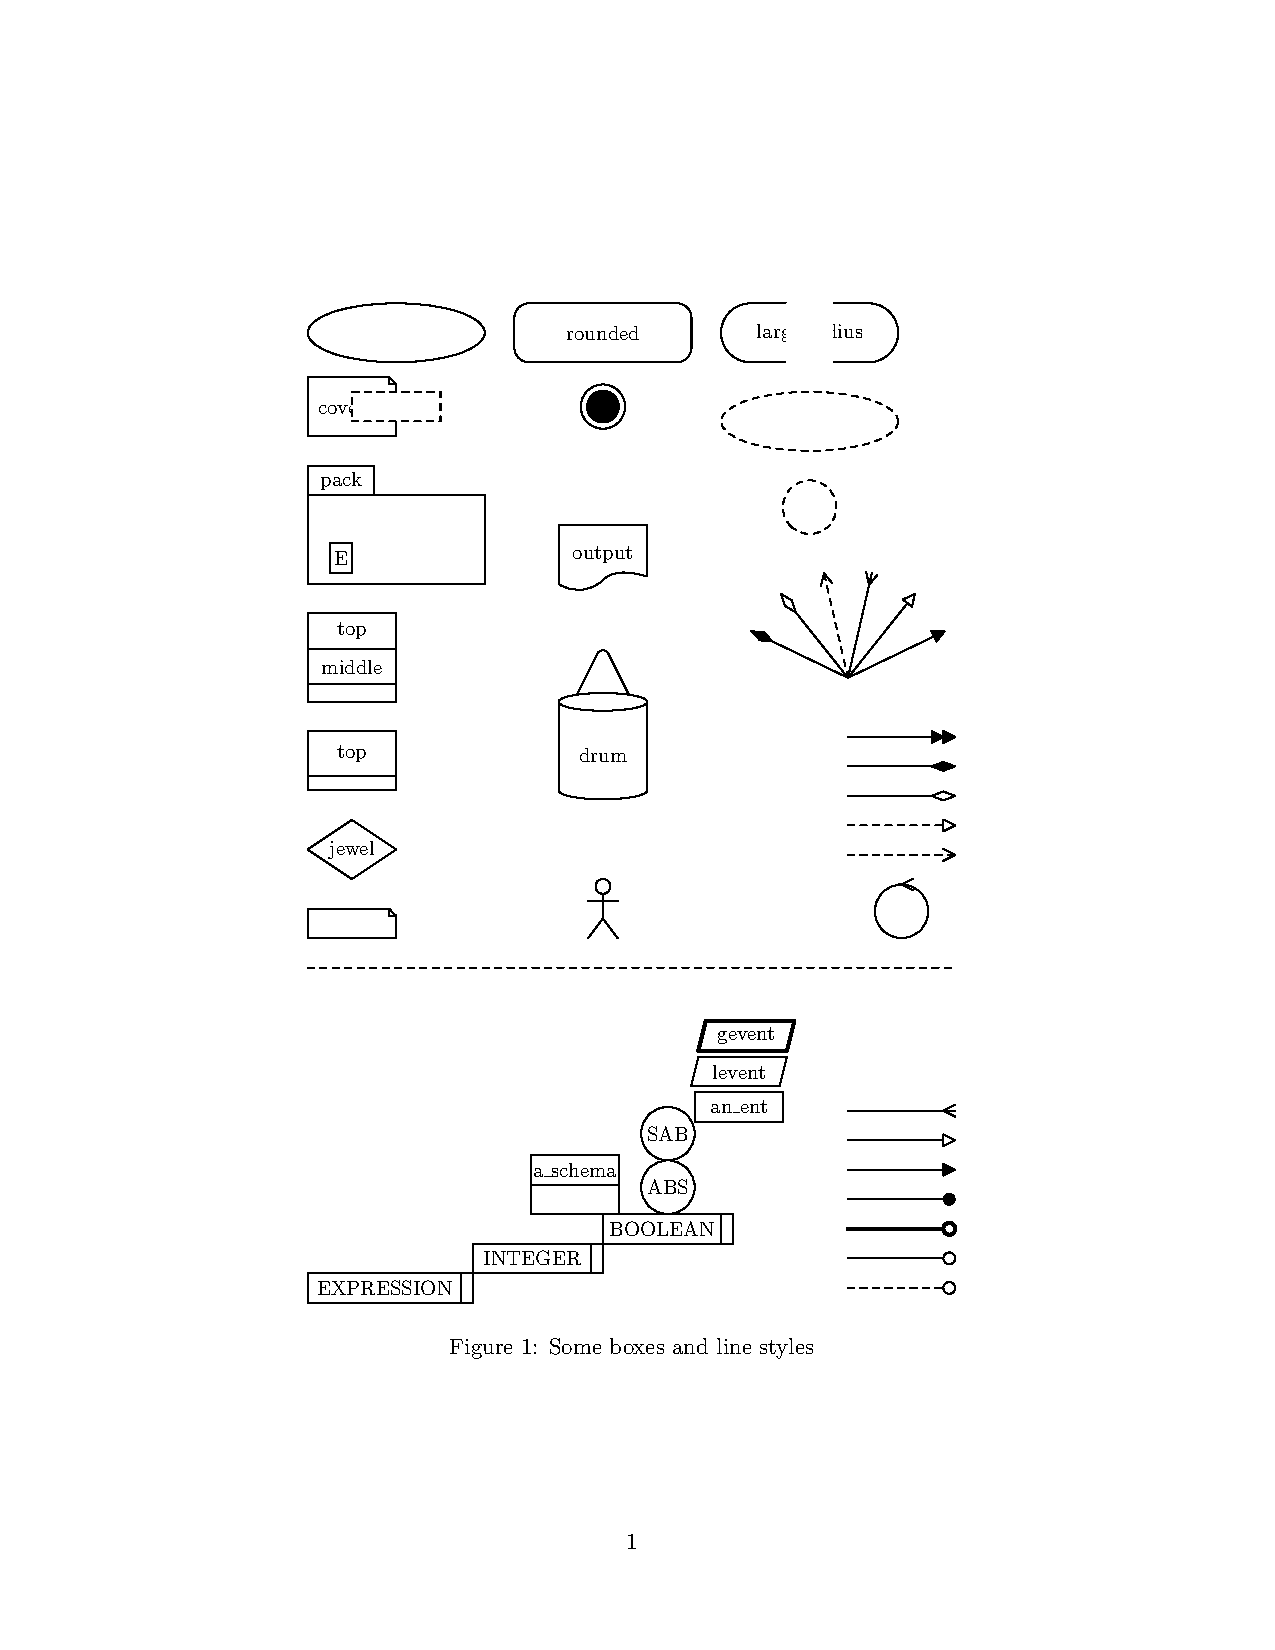
\includegraphics{expeg.4}
\caption{Supertypes and subtypes}
\end{figure}

\begin{figure}
\centering
  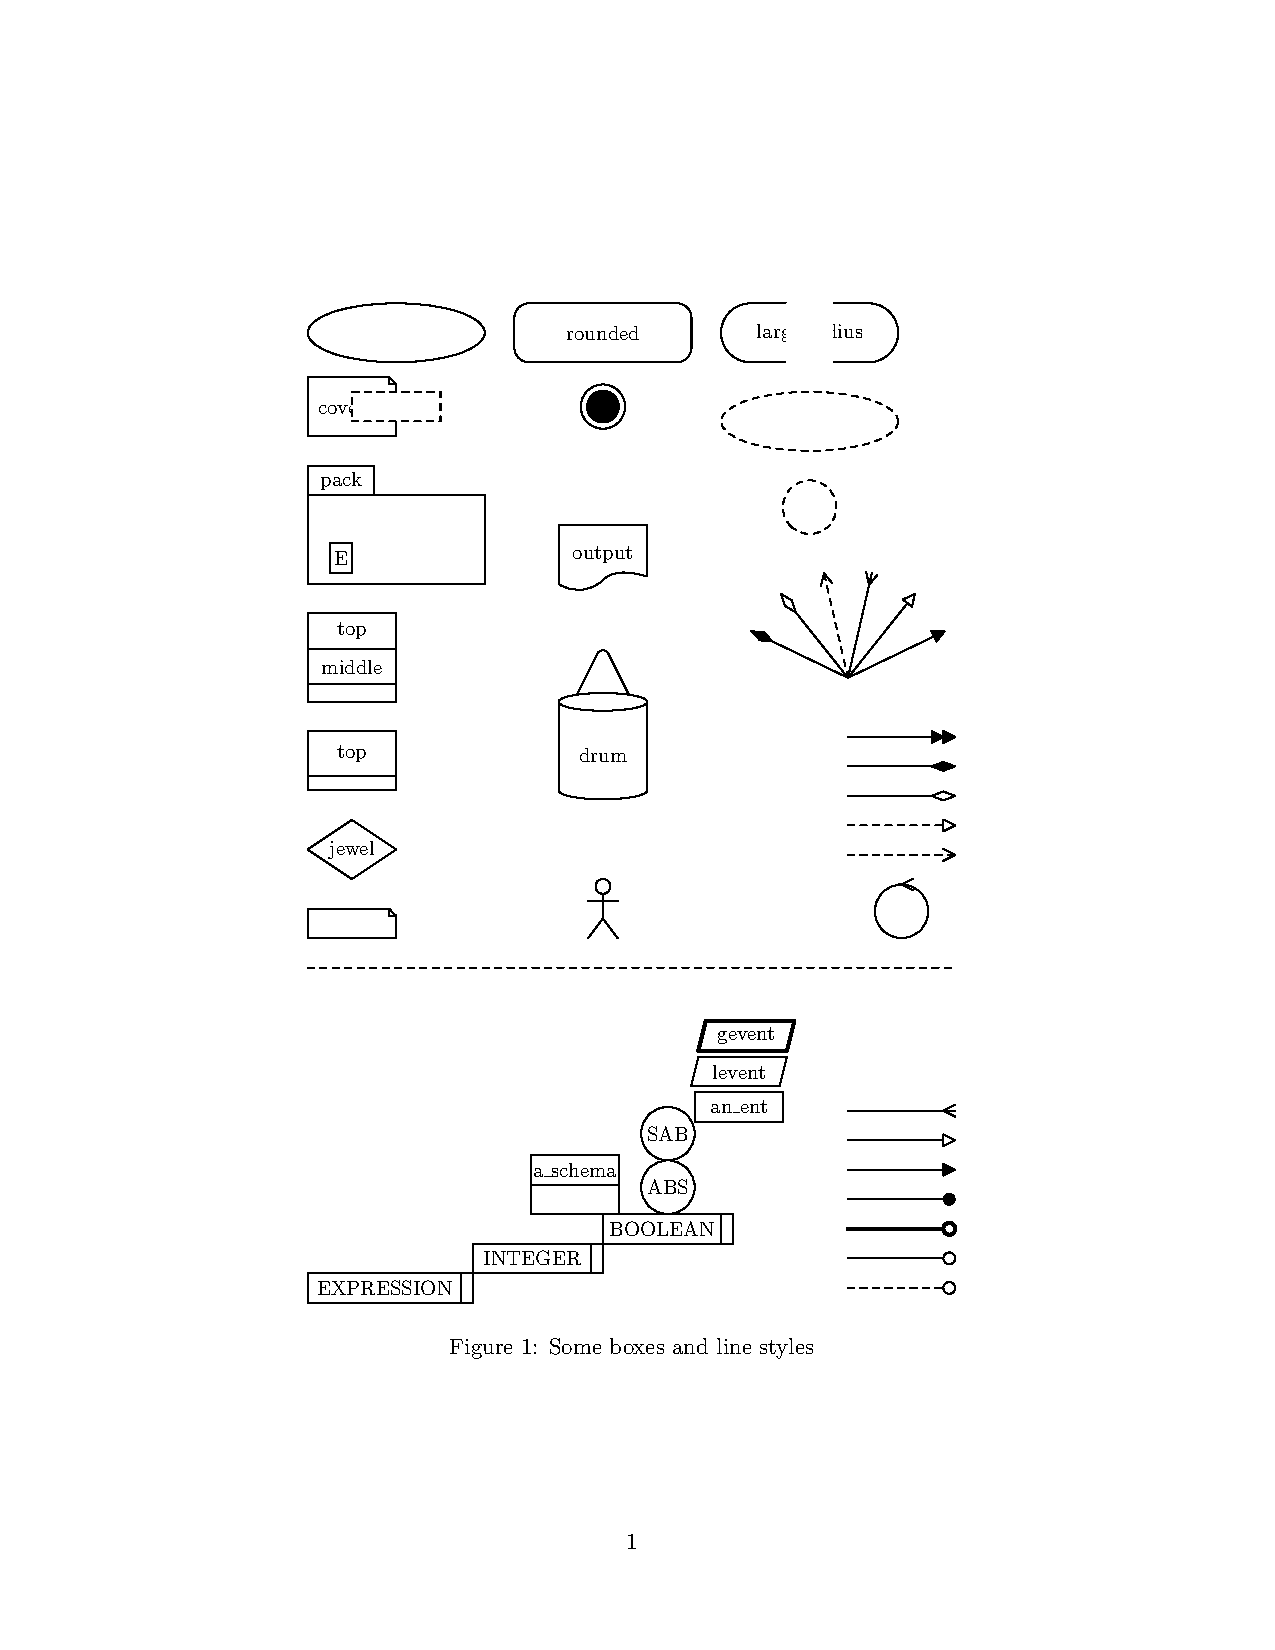
\includegraphics{expeg.5}
\caption{A portion of a large model}
\end{figure}

\begin{figure}
\centering
  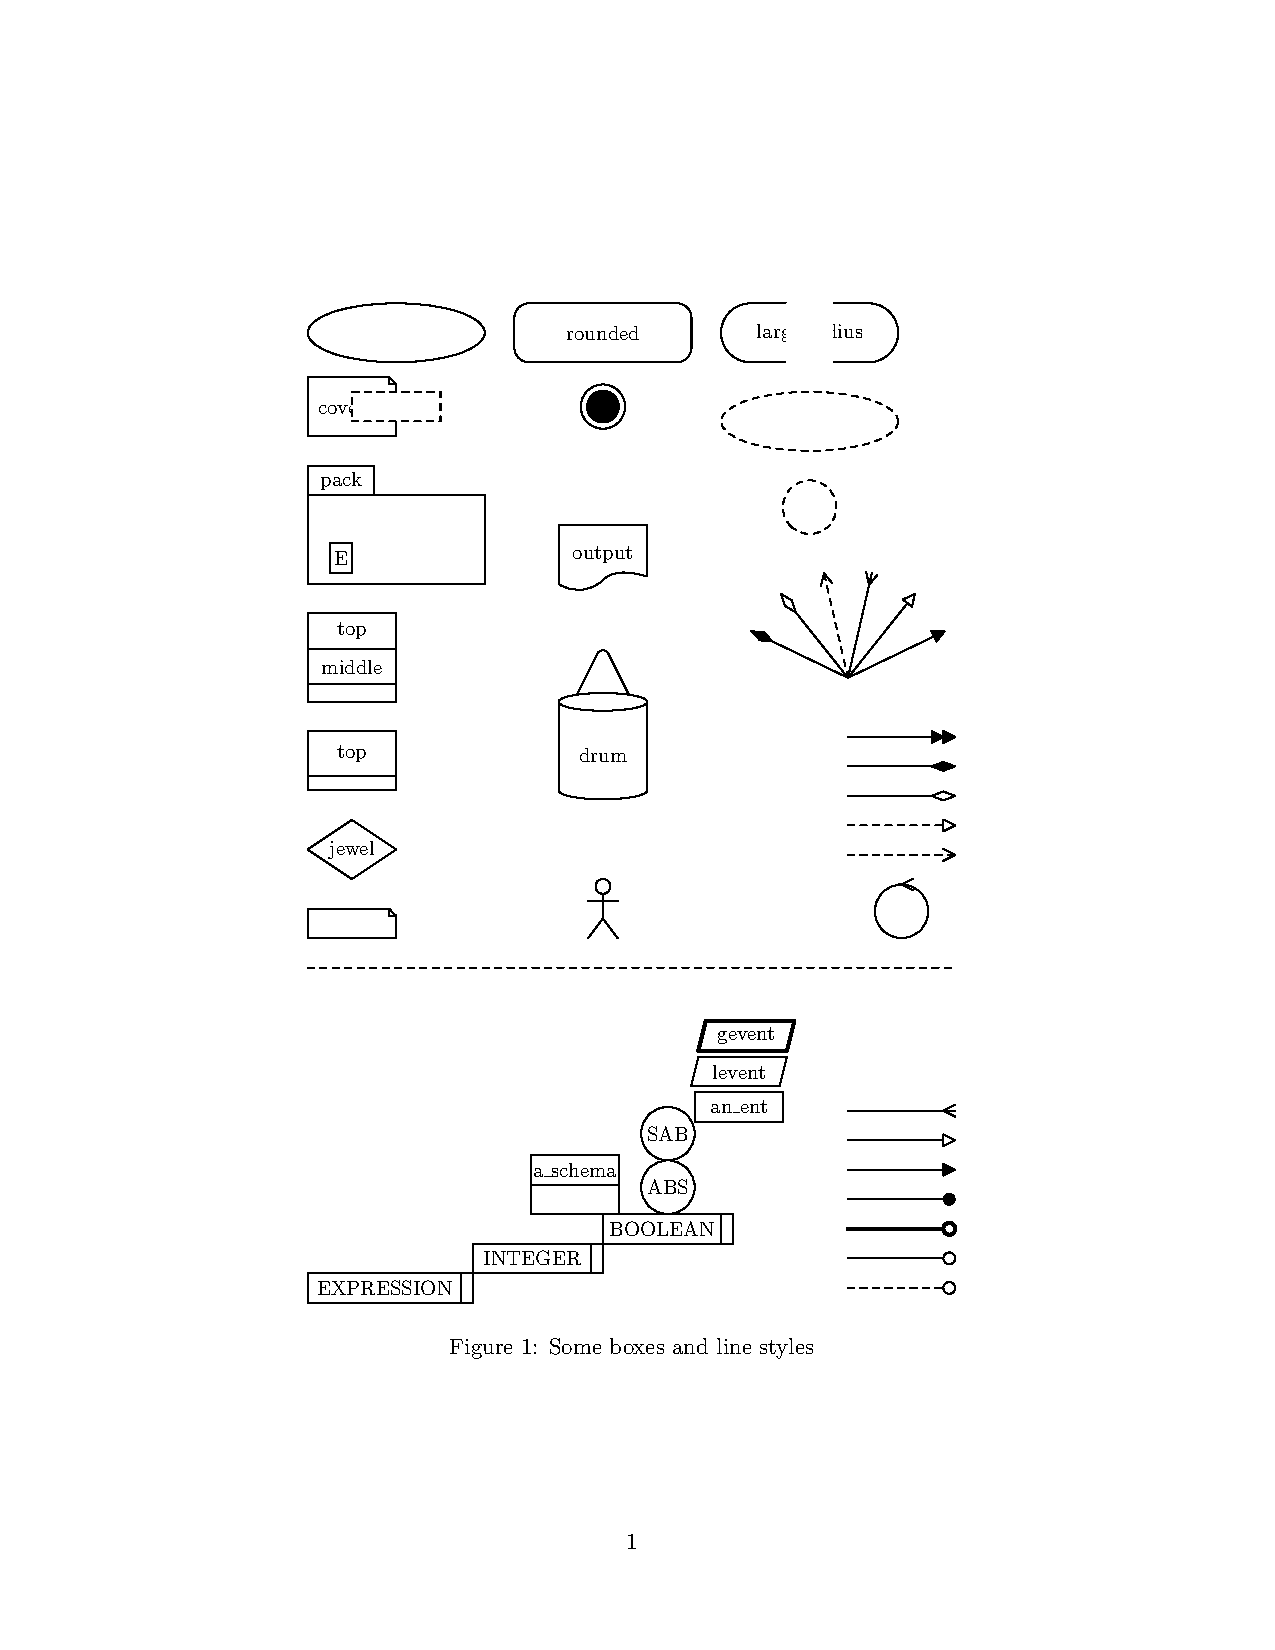
\includegraphics{expeg.6}
\caption{Car model using EXPRESS-G}
\end{figure}

\begin{figure}
\centering
  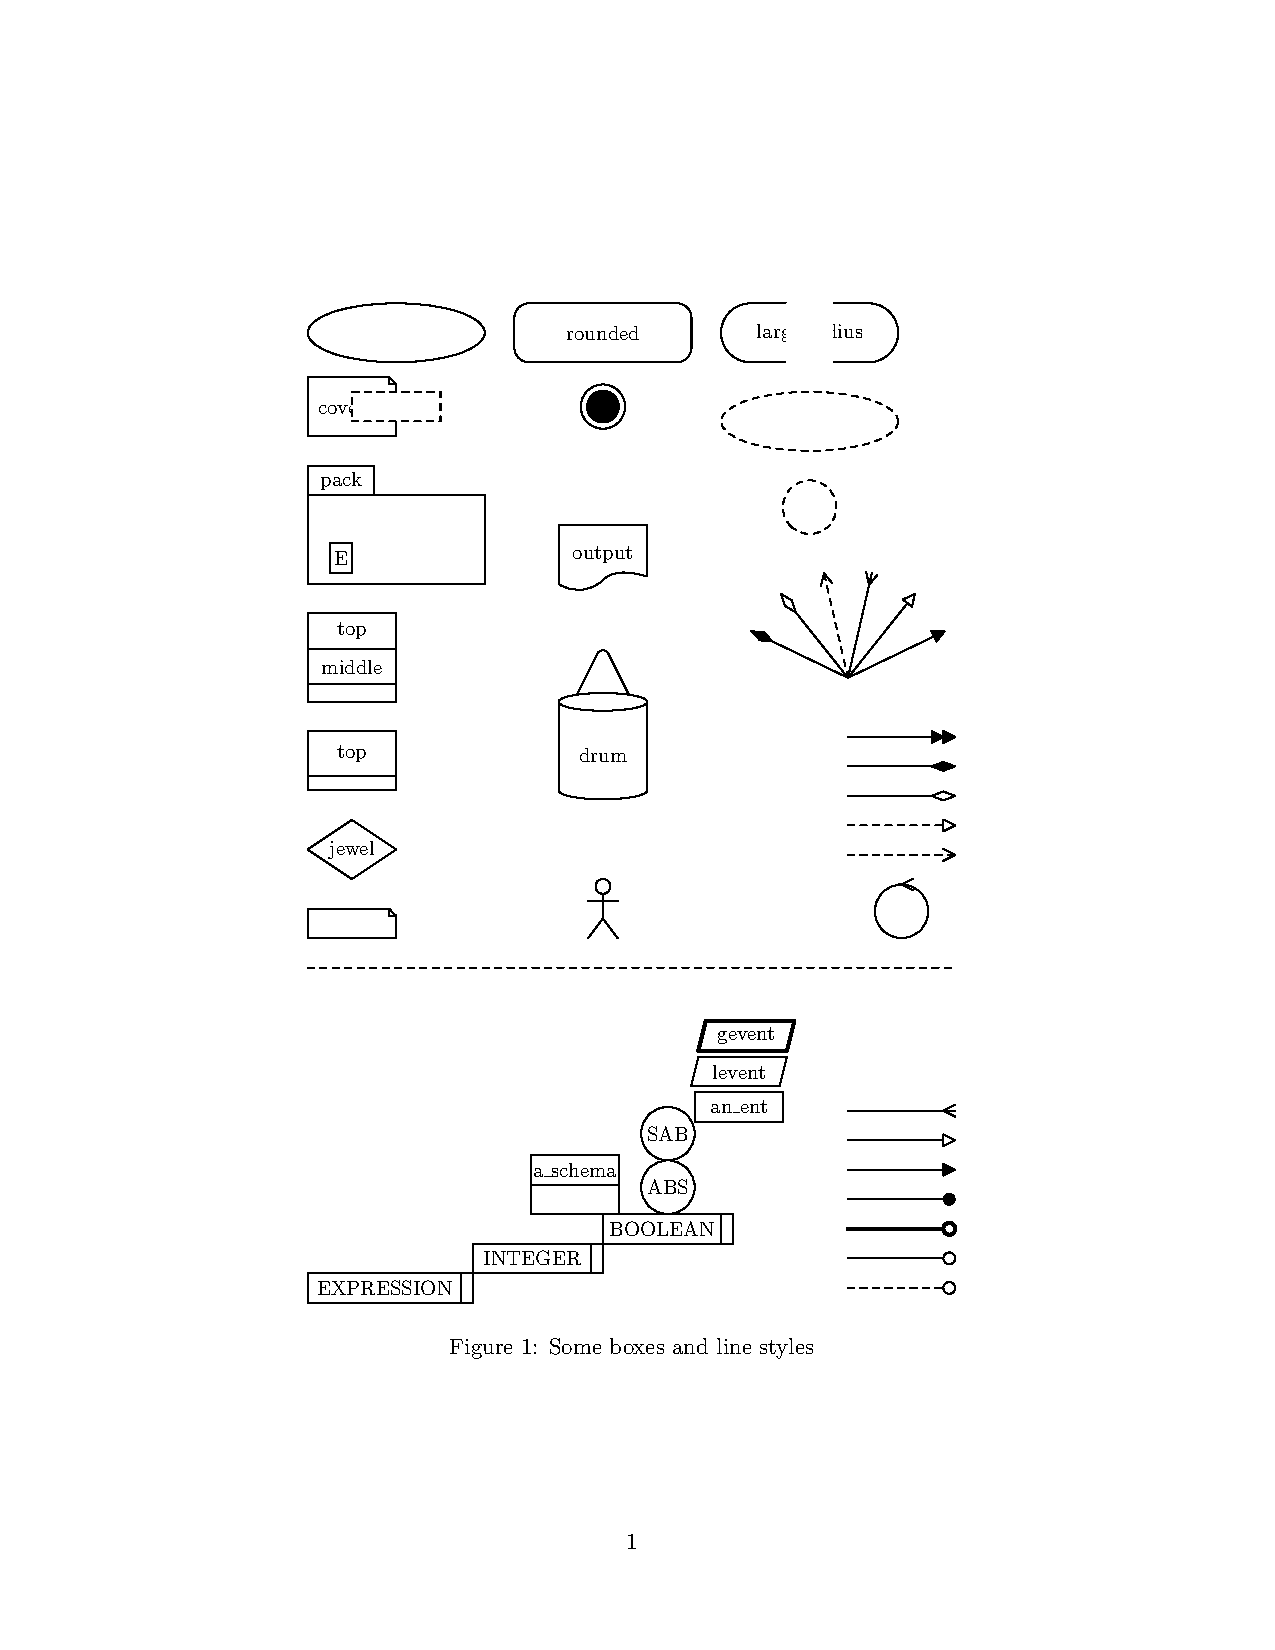
\includegraphics{expeg.7}
\caption{Car model using Shlaer-Mellor}
\end{figure}

\begin{figure}
\centering
  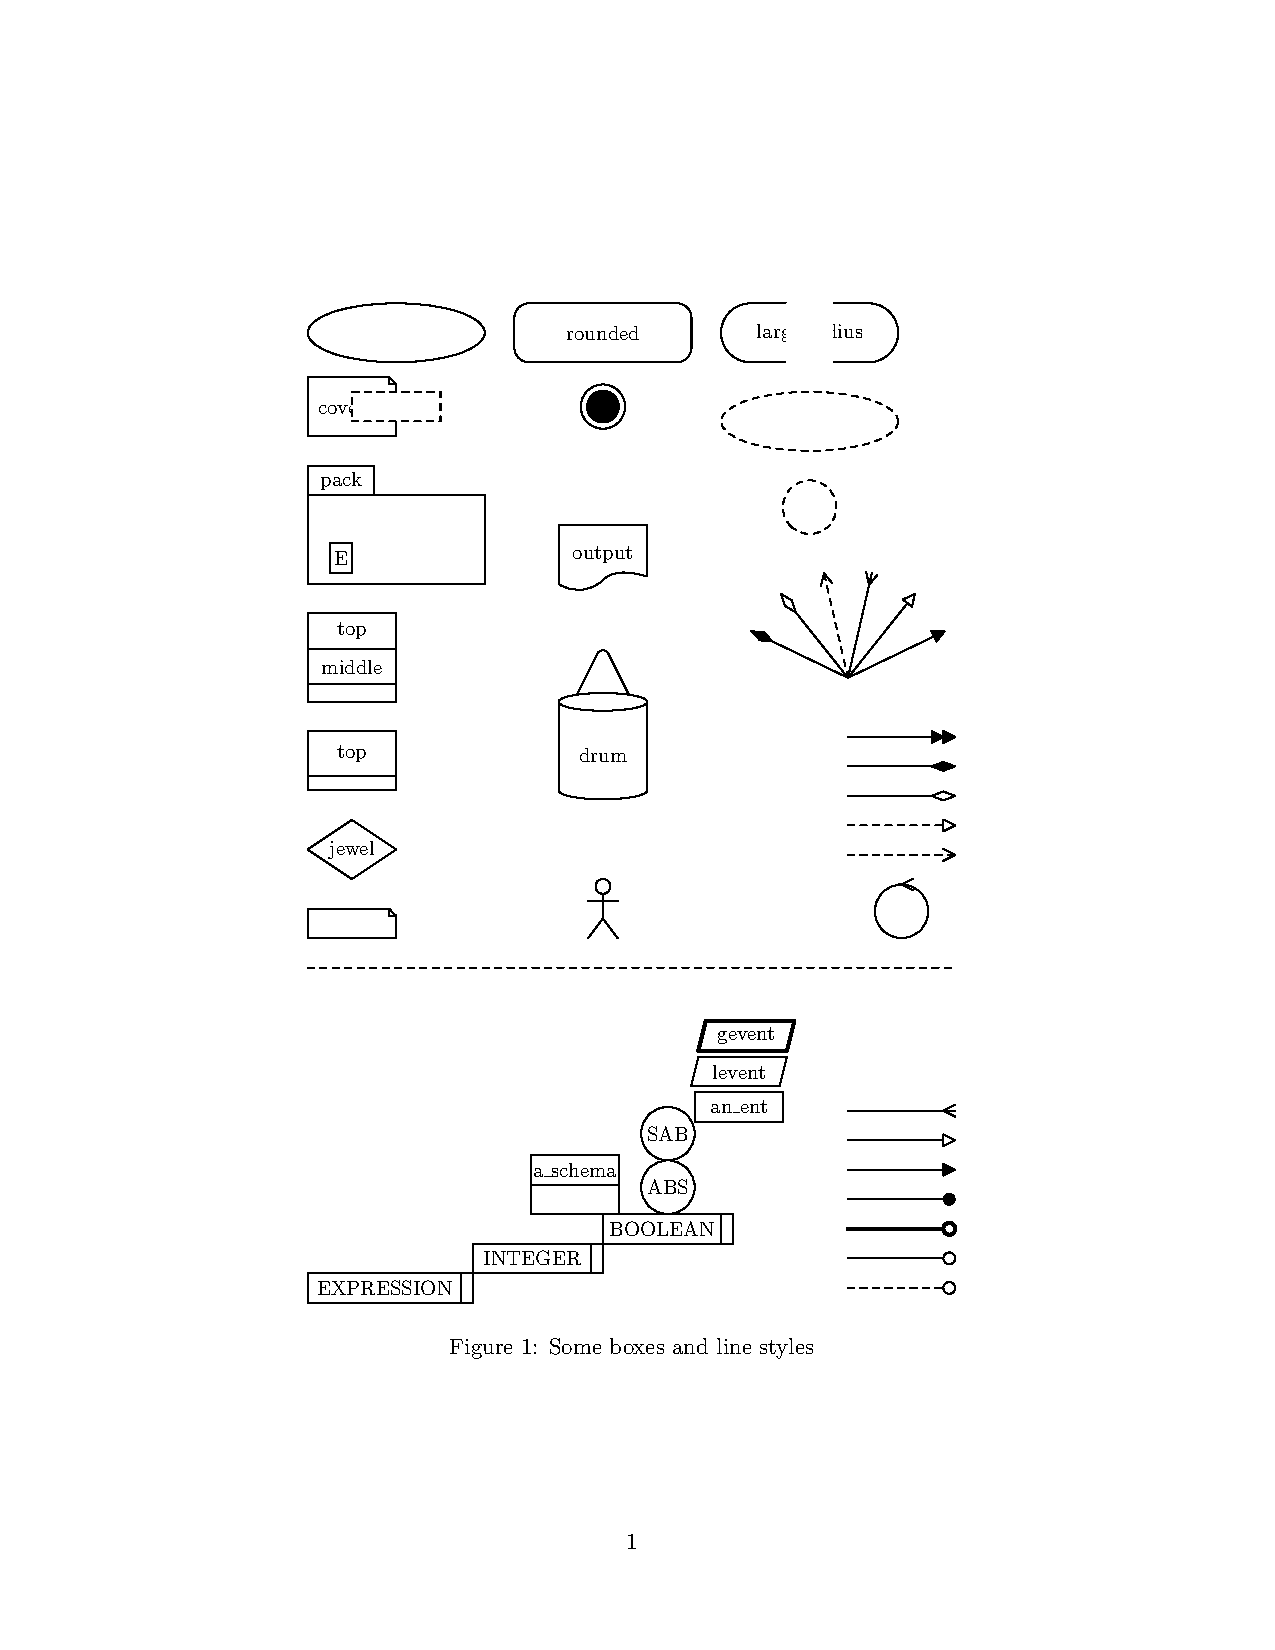
\includegraphics{expeg.8}
\caption{Car model using IDEF1X}
\end{figure}

\begin{figure}
\centering
  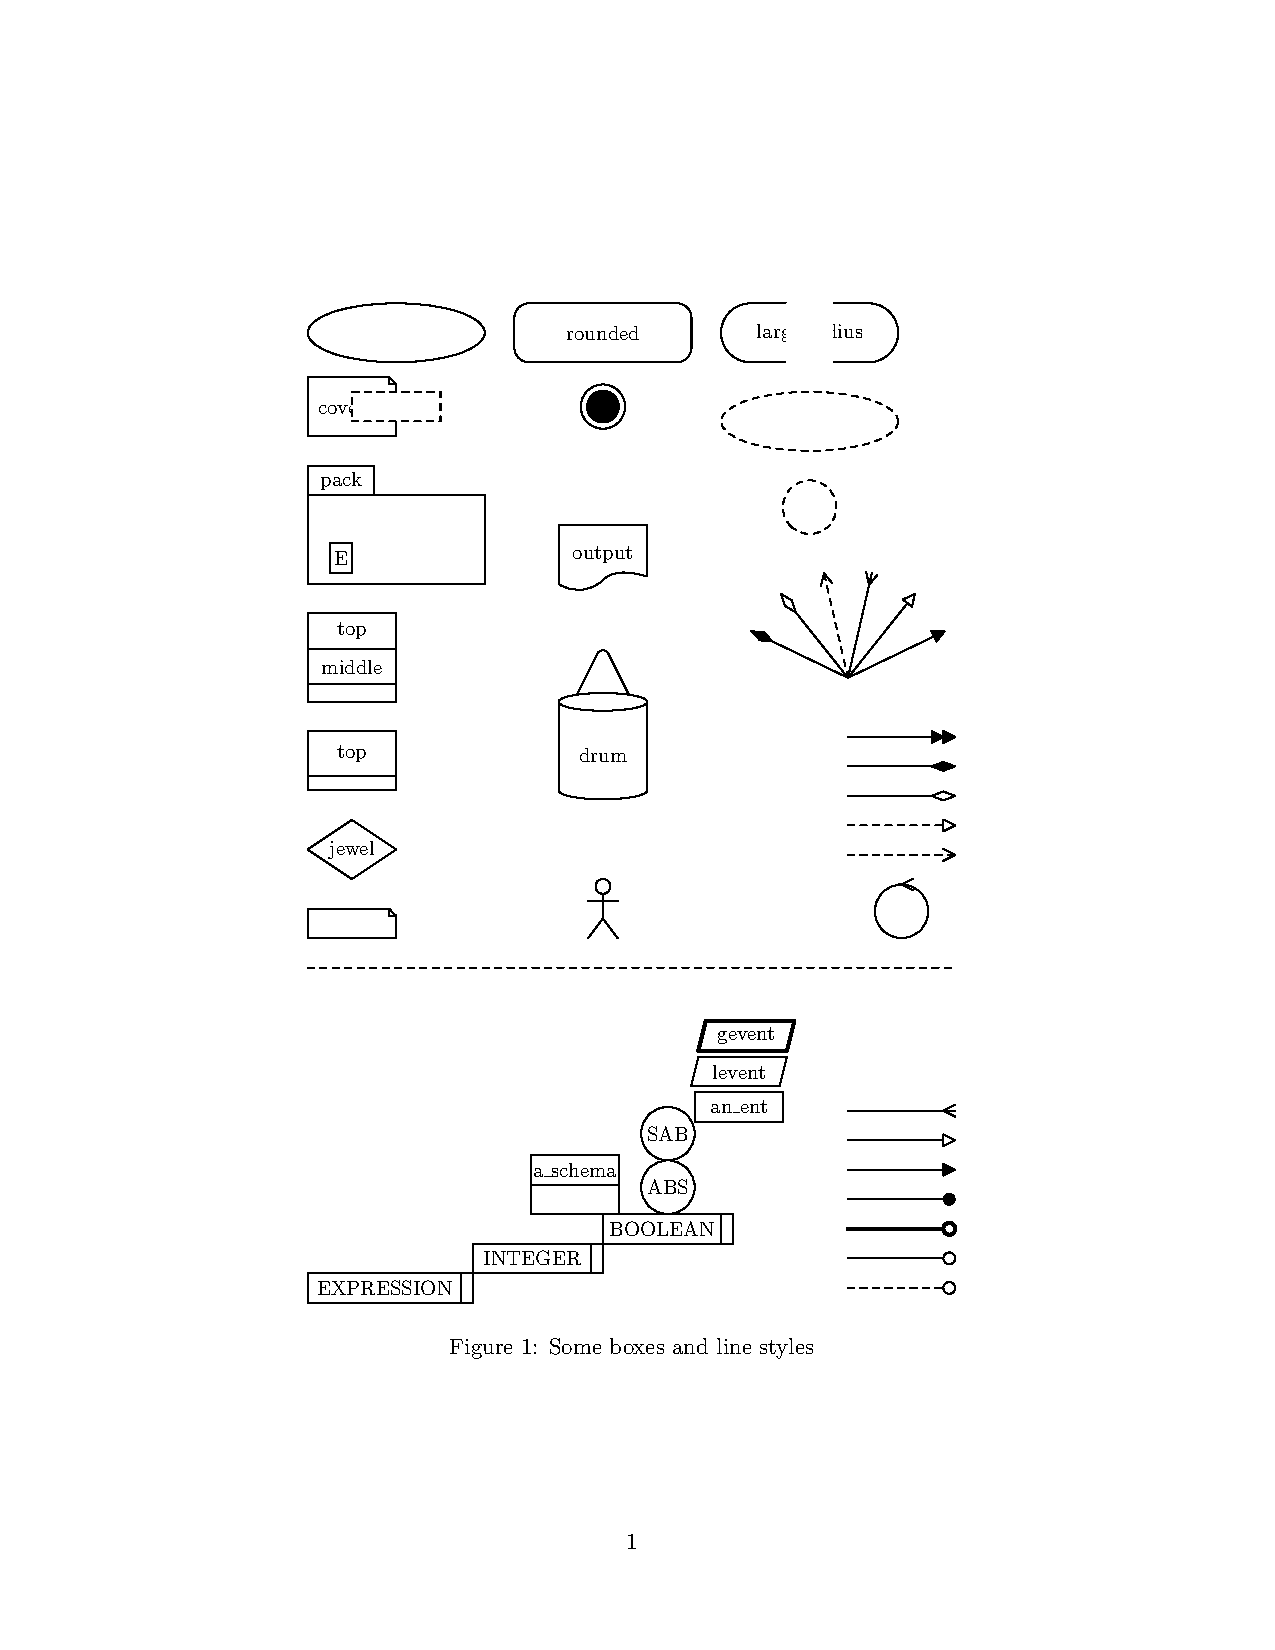
\includegraphics{expeg.9}
\caption{Car model using OMT}
\end{figure}

\begin{figure}
\centering
  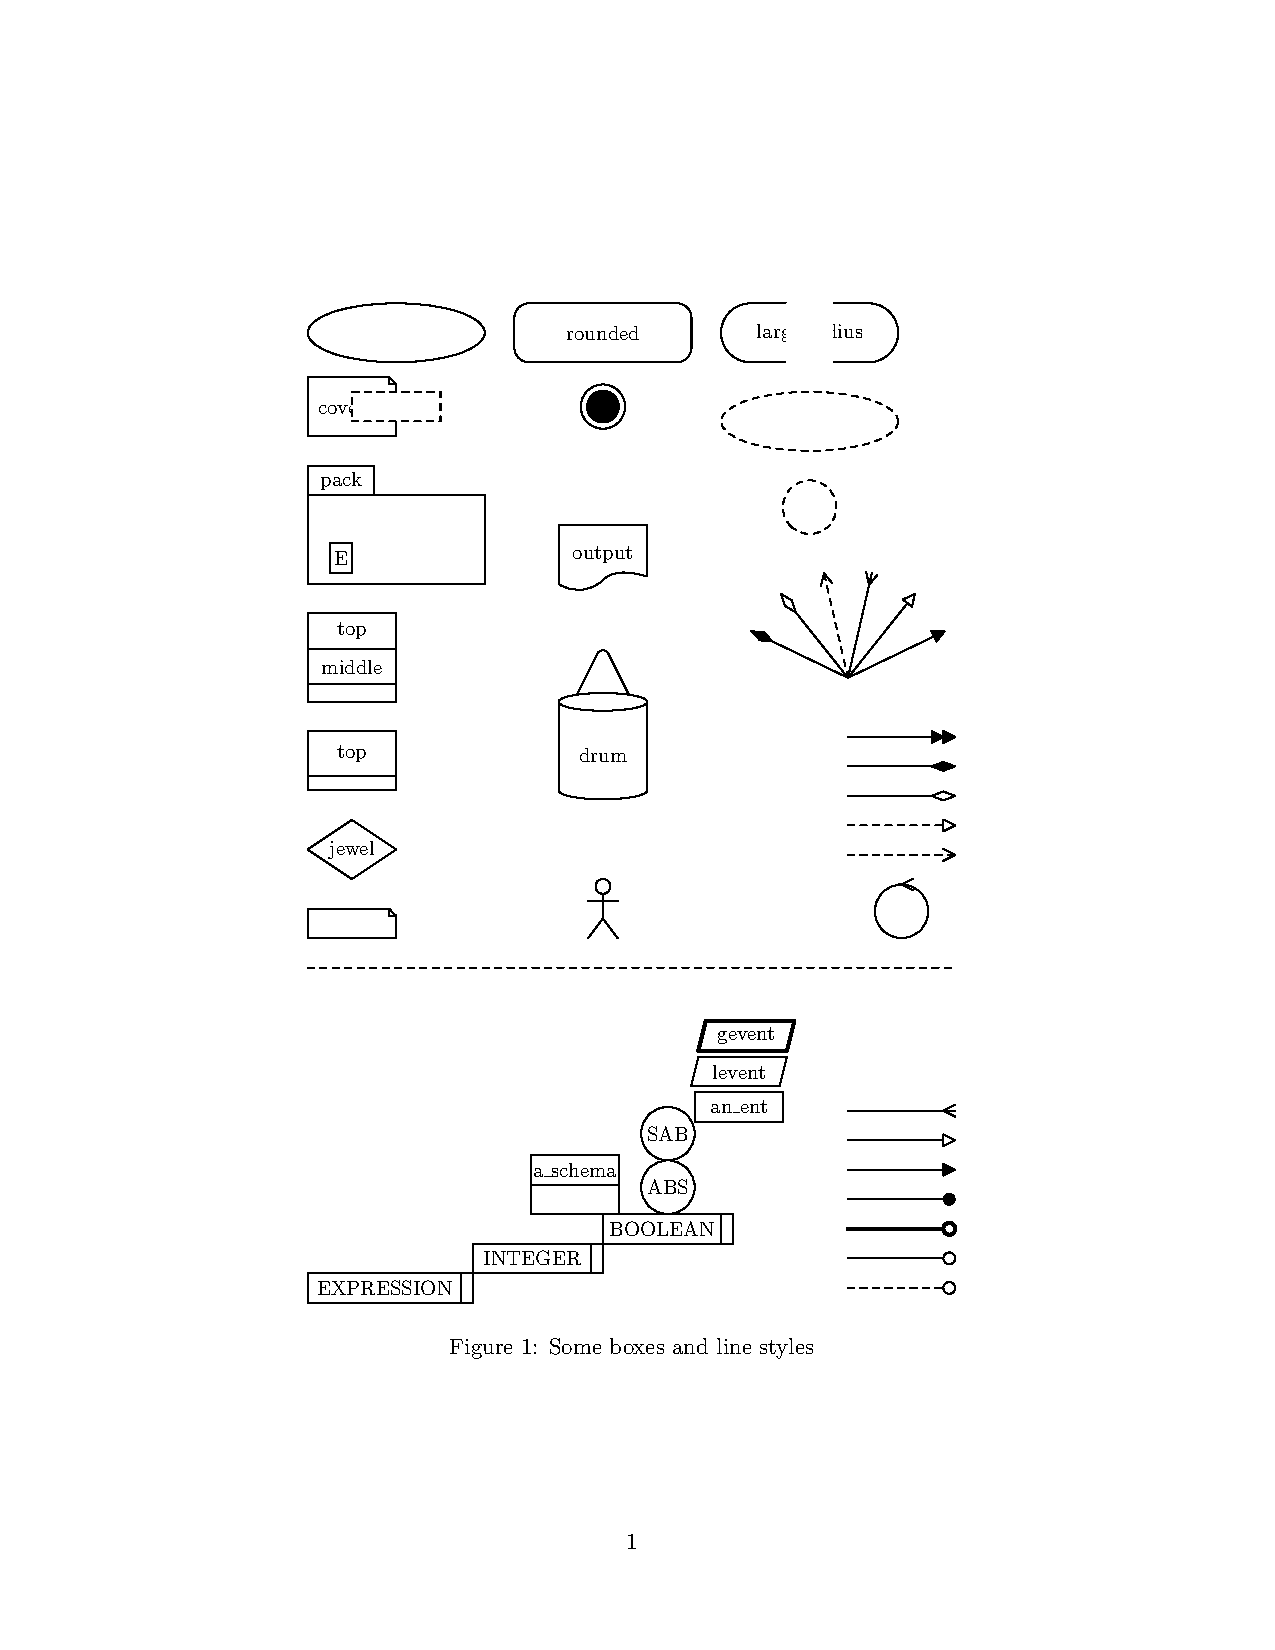
\includegraphics{expeg.10}
\caption{Car model using E-R}
\end{figure}

\begin{figure}
\centering
  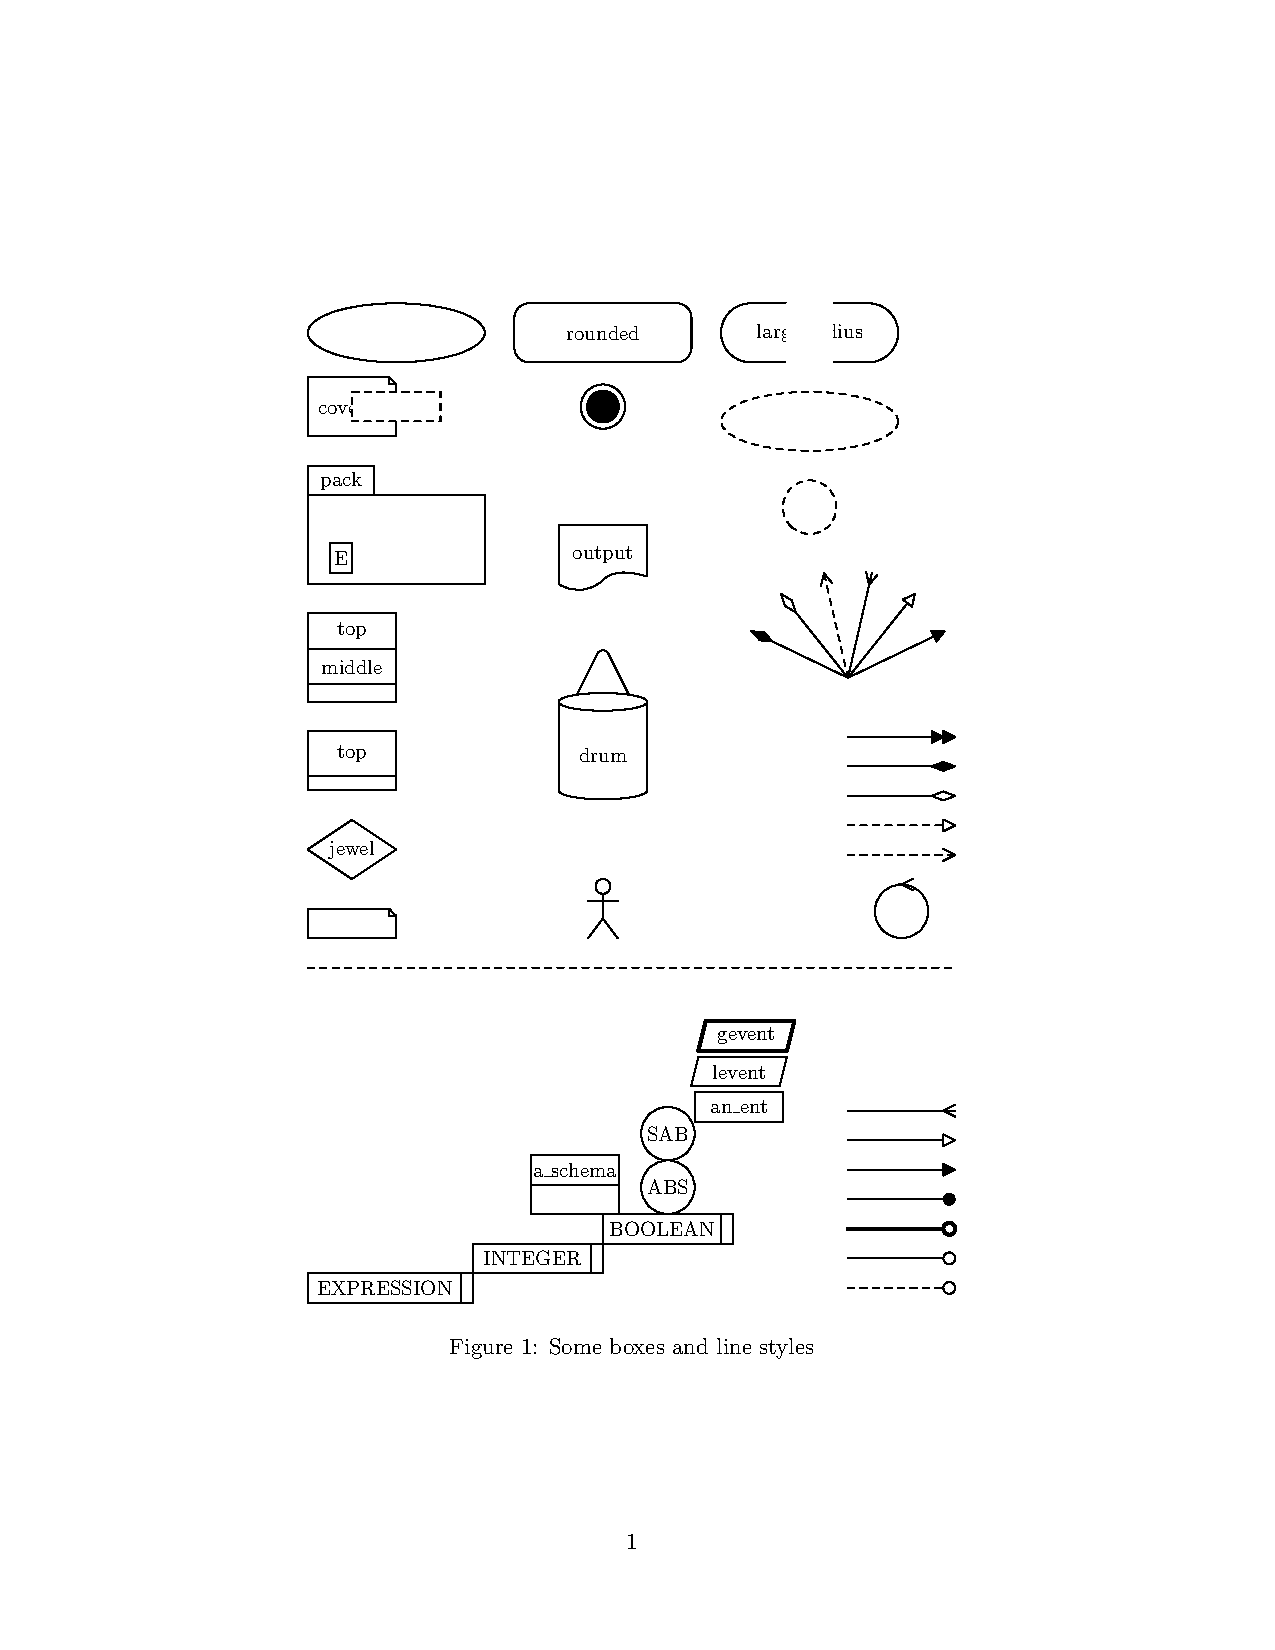
\includegraphics{expeg.11}
\caption{Car model using NIAM}
\end{figure}

\end{document}

\endinput
%%
%% End of file `expeg.tex'.
